\chapter{Theory of Debt, Its Proper Role, and Leverage Cycles}

This chapter follows Robert J. Shiller's eighth lecture in Yale's \textit{Financial Markets} course, curated for the LazyingArt LLC track. The lecture is explicitly split in two. We do the technical things first: an Irving Fisher model of interest, present value, discount bonds, compounding, conventional bonds, the term structure, and forward rates. Only after that do we return to the larger question of what debt markets are really doing in social life. That order matters. The mathematics is introduced as groundwork for judgment, not as a substitute for it. The opening puzzle is therefore a serious one: why are interest rates positive at all, and why do they so often sit at only a few percent per year?

\section{Why interest rates need an explanation}

An interest rate is the percentage one earns on a loan or pays on a loan, depending on which side of the contract one stands. The lecture begins by insisting that we not treat that as a trivial fact. Interest rates are ancient. They have existed for thousands of years. They are usually positive. They are often in the neighborhood of a few percent. Why should that be so? Why not zero? Why not negative? Why not something drastically larger?

Shiller begins, not with a pricing formula, but with the history of thought. In Bohm-Bawerk's late nineteenth-century account, the rate of interest is explained in broad verbal terms by three causes.

\begin{itemize}
\item Technical progress: as knowledge accumulates, future production may be better than present production.
\item Roundaboutness: production that takes time, including indirect methods and tool-making, may be more productive than direct production.
\item Time preference: people may prefer present consumption to future consumption; that is, they may be impatient.
\end{itemize}

The important point is that this is still literary economics. It is suggestive and powerful, but it is not yet a model that places these causes inside one clear mechanism. Fisher's contribution is to take this loose verbal list and convert it into a disciplined two-period equilibrium picture.

\section{From Bohm-Bawerk to Fisher's two-period framework}

Shiller briefly acknowledges the textbook summary associated with Fisher: the interest rate may be drawn as the intersection of a supply curve and a demand curve for savings. The supply of saving slopes upward because higher rates induce more people to save. The demand for investment funds slopes downward because lower rates make borrowing more attractive to businesses. This is not wrong. But it is too compressed for the lecture's purpose.

So we move to Fisher's more revealing diagram. Shiller lingers over the historical fact that Fisher was a Yale professor and even remarks that one can imagine Fisher lecturing from the same blackboard. The point of the historical setup is not nostalgia. It is that Fisher's 1930 \textit{Theory of Interest} provides a diagram that brings Bohm-Bawerk's causes together more succinctly than the textbook supply-and-demand cross.

\begin{figure}[t]
\centering

\includegraphics[width=0.82\textwidth]{lecture_08_figure_02.png}
\caption{Irving Fisher board and cropped two-period diagram. The screenshot fixes the historical framing; the transcript supplies the economic labels and the logic of the geometry.}
\end{figure}

The axes are current consumption and next year's consumption. To animate them, Shiller tells a Robinson Crusoe story. Crusoe has grain. He must decide how much to consume this year and how much to save and plant for next year. If total current grain endowment is \(e\), current consumption is \(c_0\), and next year's consumption is \(c_1\), then in a cleaned notation consistent with the lecture's linear technology story we may write
\begin{equation}
c_1=(1+r)(e-c_0).
\end{equation}
The slope of the production possibility frontier is therefore
\begin{equation}
\frac{dc_1}{dc_0}=-(1+r).
\end{equation}
Shiller says on the board that the slope is ``minus 1 plus \(r\).'' In the notes it is best to normalize that to the standard form \( -(1+r)\).

The first Fisher story is intentionally simple. For every bushel of grain planted, Crusoe may get two bushels next year. In that stripped-down case, \(1+r=2\). The frontier is a straight line. Crusoe still chooses a point on it by comparing present and future consumption, and the difference between his endowment and his current consumption is saving. But if the frontier is linear, the interest rate itself is pinned down by technology. Preferences determine where he lives on the line, not the line's slope. So impatience has not yet fully entered the rate of interest.

That is why the lecture immediately takes the next step.

\section{Robinson Crusoe, first alone and then in a loan market}

The next step is diminishing returns. If Crusoe plants only a little grain, he may use the best land and do very well. But as he saves more and more, the additional grain planted may be less productive. The production possibility frontier then bends inward. Now the rate of interest is no longer just the slope of a straight technological opportunity set. It is the slope at the point where technology and taste meet.

\begin{figure}[t]
\centering
\begin{tikzpicture}[scale=1.0]
\draw[->] (0,0) -- (6.2,0) node[below] {$c_0$};
\draw[->] (0,0) -- (0,5.2) node[left] {$c_1$};
\draw[thick] (0.4,4.7) .. controls (1.2,4.55) and (3.4,3.15) .. (5.3,0.4);
\draw[dashed] (0.75,4.3) -- (5.8,1.05);
\draw[thick] (0.65,4.15) .. controls (1.8,3.85) and (3.35,2.75) .. (5.0,1.5);
\fill (5.3,0.4) circle (1.5pt) node[below right] {$e$};
\fill (2.95,2.85) circle (1.5pt) node[above right] {$P^\ast$};
\node at (4.8,4.25) {PPF};
\node at (4.75,2.25) {$u^\ast$};
\node at (4.15,0.8) {$-(1+r)$};
\end{tikzpicture}
\caption{Cleaned reconstruction of Fisher's one-person two-period geometry after diminishing returns are introduced. The cropped board confirms the presence of the graph; the transcript supplies the economic structure.}
\end{figure}

Crusoe chooses the highest indifference curve tangent to the production possibility frontier. At that tangency,
\begin{equation}
\mathrm{MRS}_{c_0,c_1}=\mathrm{MRT}_{c_0,c_1}=1+r.
\end{equation}
Now we can finally say what Fisher adds to Bohm-Bawerk. Roundaboutness and productivity are carried by the frontier. Technical progress can shift the frontier itself. Time preference appears in the slope and shape of the indifference curves. The interest rate is therefore not just impatience and not just productivity. It is the slope at a tangency between the two.

This also yields the lecture's comparative statics. Suppose Crusoe becomes more impatient. Then he wants more consumption today and less next year. The tangency moves to the right. Because it moves to a steeper part of the frontier, the implied interest rate rises. If, instead, Crusoe is very patient, the tangency lies further up and to the left, and the implied interest rate is lower. So impatience matters, but only through its interaction with the production frontier.

At that point Shiller recaps: we now have all of Bohm-Bawerk's causes. But he is not satisfied yet. A one-person economy has no trade. So he adds a second Crusoe.

The second stage is the lending market. There are now two Crusoes on opposite sides of the island. They have the same technology and the same endowment, but not the same patience. One wants more consumption today and saves little. The other is patient and saves heavily for the future. If they remain isolated, they choose different tangencies on the same frontier. But once they discover each other, there are gains from trade.

The reason is not merely that tastes differ. It is that the patient Crusoe is planting so much that he is deep into diminishing returns, while the impatient Crusoe is planting relatively little, where marginal productivity is still high. A loan transfers grain toward the more productive use and simultaneously moves both agents toward preferred consumption plans.

\begin{figure}[t]
\centering
\begin{tikzpicture}[scale=1.0]
\draw[->] (0,0) -- (6.2,0) node[below] {$c_0$};
\draw[->] (0,0) -- (0,5.2) node[left] {$c_1$};
\draw[thick] (0.4,4.7) .. controls (1.4,4.45) and (3.5,3.15) .. (5.35,0.4);
\draw[dashed] (0.6,4.35) -- (5.85,0.95);
\fill (3.0,2.8) circle (1.5pt) node[above right] {$P$};
\fill (4.45,1.86) circle (1.5pt) node[right] {$A$};
\fill (1.85,3.54) circle (1.5pt) node[left] {$B$};
\draw[thick] (3.0,3.15) .. controls (3.45,2.85) and (3.95,2.3) .. (5.15,1.66);
\draw[thick] (0.95,3.95) .. controls (1.25,3.9) and (1.55,3.72) .. (2.75,3.0);
\node at (4.9,4.25) {PPF};
\node at (4.85,2.55) {$u_A$};
\node at (1.2,3.2) {$u_B$};
\end{tikzpicture}
\caption{Two Crusoes with different patience. Production occurs at the common tangent point \(P\), while lending supports different consumption points \(A\) and \(B\) on the same intertemporal line.}
\end{figure}

The market interest rate is the slope of the common tangent line. That is the lecture's central theoretical statement. The interest rate is not read off from any one person's impatience. It emerges from heterogeneous preferences interacting with a common technological opportunity set.

\subsection{Question \& Answer}

\paragraph{Question.} Why is a loan socially useful in the Fisher story?

\paragraph{Answer.} Because with diminishing returns and different degrees of patience, isolated production plans are inefficient. The patient Crusoe is planting too much where marginal productivity is low; the impatient Crusoe is planting too little where marginal productivity is high. A loan reallocates grain toward the more productive margin and lets both agents move to higher indifference curves. The common tangent line clears the loan market and makes both better off.

This is precisely where the lecture pauses. Put this way, lending looks obviously good. Shiller does not abandon that conclusion. He says, in effect, let us take this Fisher theory of interest as given. But before we return to criticisms of lending, we must do the arithmetic of finance.

\section{Debt arithmetic: discount bonds, compounding, and present discounted value}

Here the lecture deliberately changes level. We move from the equilibrium logic of interest to the pricing of loan instruments. The first and simplest instrument is the discount bond.

A discount bond promises a fixed payment at a future date and sells today for less than that payment. It has no coupon stream along the way. If a bond pays \(100\) at maturity \(T\), then under annual compounding its present price is
\begin{align}
p &= \frac{100}{(1+r)^T}, \\
(1+r)^T &= \frac{100}{p}, \\
r &= \left(\frac{100}{p}\right)^{1/T}-1.
\end{align}
The rate \(r\) inferred from price is the yield to maturity. The point is subtle but important: the bond itself is quoted as a price, but we can back out an annual interest rate from that price once maturity and compounding are specified.

\paragraph{Worked calculation.} For a two-year discount bond,
\begin{equation}
p=\frac{100}{(1+r)^2}
\qquad\Longrightarrow\qquad
r=\sqrt{\frac{100}{p}}-1.
\end{equation}
This is the simplest explicit bridge from bond price to interest rate.

Shiller then stops and carefully distinguishes compounding conventions. Under annual compounding, interest is credited once per year. If one deposits \(B_0\) today, then after \(T\) years the balance is
\begin{equation}
B(T)=B_0(1+r)^T.
\end{equation}
But finance often prefers semiannual conventions, because conventional bonds pay coupons every six months. The transcript's notation becomes unstable here, so it is best to normalize it once:
\begin{equation}
z=\frac{r}{2}, \qquad n=2T, \qquad p=\frac{100}{(1+z)^n},
\end{equation}
where \(z\) is the half-year rate and \(n\) counts half-year periods.

\begin{figure}[t]
\centering

\includegraphics[width=0.82\textwidth]{lecture_08_figure_03.png}
\caption{Annual versus continuous compounding on the board. The screenshot matters because it preserves the comparative board layout, not just the final exponential term.}
\end{figure}

The lecture then takes the limiting case: compound more and more frequently until compounding becomes continuous. The full sentence on the board is partly obscured, but the standard completion consistent with the lecture is
\begin{equation}
B(T)=B_0 e^{rT}.
\end{equation}
So annual compounding and continuous compounding are not two unrelated formulas. They are two versions of the same intertemporal calculation under different conventions.

\paragraph{Present discounted value.} This is the central technical concept of the middle of the lecture. If a single payment \(x\) arrives at date \(T\), then under annual compounding
\begin{equation}
\mathrm{PDV}=\frac{x}{(1+r)^T}.
\end{equation}
If annual payments \(\{x_t\}\) arrive over time, then
\begin{equation}
\mathrm{PDV}=\sum_{t=1}^{\infty}\frac{x_t}{(1+r)^t}.
\end{equation}
If payments arrive every six months, the corresponding semiannual expression is
\begin{equation}
\mathrm{PDV}=\sum_{t=1}^{\infty}\frac{x_t}{(1+r/2)^t}.
\end{equation}
And if payments arrive continuously, then the sum becomes an integral:
\begin{equation}
\mathrm{PDV}=\int_0^\infty x(t)e^{-rt}\,dt.
\end{equation}

Shiller emphasizes that this is what finance repeatedly does. It takes many future payments and turns them into one present number. Once that number has been computed, very different instruments can be compared on a common basis.

\section{Perpetuities, annuities, and conventional bonds}

Now the board becomes formula-dense, but the lecture still proceeds in a definite order. We do not start with the full conventional bond. We begin with the simplest infinite payment stream, then truncate it, and only then add principal repayment.

\begin{figure}[t]
\centering

\includegraphics[width=0.82\textwidth]{lecture_08_figure_04.png}
\caption{Annuity setup beside the consol benchmark. The screenshot preserves the moment when the lecture moves from the perpetuity formula to the finite annuity case.}
\end{figure}

A consol, or perpetuity, pays the same coupon forever. The board writes the special case of a one-pound coupon:
\begin{equation}
\mathrm{PDV}_{\text{consol}}=\frac{\pounds 1}{r}.
\end{equation}
In normalized form we write
\begin{equation}
\mathrm{PDV}_{\text{consol}}=\frac{C}{r},
\qquad
r=\frac{C}{\mathrm{PDV}_{\text{consol}}}.
\end{equation}
This is the benchmark against which the annuity is introduced.

An annuity is a finite payment stream. It pays \(x\) each period from \(t=1\) to \(t=T\), where \(T\) is the last payment date. The lecture writes the final formula on the board, but its logic is especially clear if we derive it from the consol. An annuity is just a perpetuity with its tail removed:
\begin{align}
\mathrm{PDV}_{\text{annuity}}
&= \frac{x}{r}-\frac{x}{r(1+r)^T} \\
&= \frac{x}{r}\left(1-\frac{1}{(1+r)^T}\right).
\end{align}
That is the formula Shiller arrives at in the annuity panel. It is important not only as algebra but as a building block. The lecture's concrete example is the traditional home mortgage: fixed payments for a finite horizon and then no more.

\begin{figure}[t]
\centering

\includegraphics[width=0.82\textwidth]{lecture_08_figure_05.png}
\caption{Finite-annuity formula applied to a conventional bond. The board makes visible both the formula and its immediate reuse for bond coupons.}
\end{figure}

The final step in this pricing sequence is the conventional bond. A conventional bond pays coupon \(C\) every six months and then pays principal at maturity together with the final coupon. The board states the decomposition more clearly than the full algebra, so we write the normalized formula cautiously:
\begin{equation}
\mathrm{PDV}_{\text{bond}}=
\frac{C}{z}\left(1-\frac{1}{(1+z)^n}\right)+\frac{F}{(1+z)^n},
\qquad
z=\frac{r}{2}, \quad n=2T.
\end{equation}
The first term is the coupon annuity. The second is the discounted principal. This is exactly the lecture's conceptual point: a conventional bond is an annuity plus a discount bond.

\begin{figure}[t]
\centering
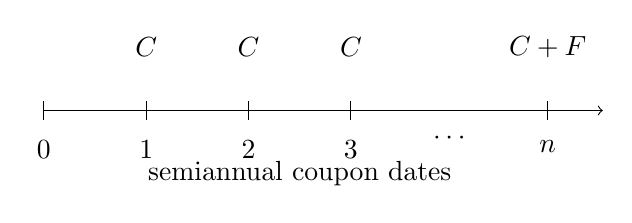
\begin{tikzpicture}[scale=1.0]
\draw[->] (0,0) -- (7.1,0);
\draw (0,0.12) -- (0,-0.12) node[below=4pt] {$0$};
\draw (1.3,0.12) -- (1.3,-0.12) node[below=4pt] {$1$};
\draw (2.6,0.12) -- (2.6,-0.12) node[below=4pt] {$2$};
\draw (3.9,0.12) -- (3.9,-0.12) node[below=4pt] {$3$};
\draw (6.4,0.12) -- (6.4,-0.12) node[below=4pt] {$n$};
\node at (1.3,0.8) {$C$};
\node at (2.6,0.8) {$C$};
\node at (3.9,0.8) {$C$};
\node at (5.15,-0.35) {$\cdots$};
\node at (6.4,0.8) {$C+F$};
\node at (3.25,-0.8) {semiannual coupon dates};
\end{tikzpicture}
\caption{Coupon timeline for a conventional bond. The diagram is subordinate to the board evidence, but it makes the annuity-plus-principal structure explicit.}
\end{figure}

\section{Forward rates from the term structure}

The next pivot is one of the lecture's best. We move from pricing a single stream to relating prices across maturities. Shiller motivates this through Sir John Hicks and a story about trying to identify who first formulated forward rates. Hicks's reply points, not to a heroic isolated discovery, but to coffee-hour conversations at the London School of Economics in the 1920s.

That anecdote matters because it shows what the problem was. Open the paper in 1925 and one sees yields for one year, two years, three years, and longer. Those are all rates from today to some future date. But what about the rate between two future dates, say from 1926 to 1927? Hicks's insight is that this rate need not be quoted separately. It is already implicit in the term structure observed today.

\begin{figure}[t]
\centering

\includegraphics[width=0.82\textwidth]{lecture_08_figure_06.png}
\caption{Forward-rate identity and expectations-theory trading setup. The screenshot preserves the board's mixture of algebra, dates, and trading instructions.}
\end{figure}

\subsection{Question \& Answer}

\paragraph{Question.} How can we lock in a one-year interest rate for a future year using only bonds traded today?

\paragraph{Answer.} Let \(r_1\) be today's one-year yield and \(r_2\) today's two-year yield. Suppose that in 1925 we know we will have \(\pounds 100\) available to invest in 1926, and we want to lock in now the one-year return from 1926 to 1927. The lecture's construction is to buy, in 1925,
\[
\frac{(1+r_2)^2}{1+r_1}
\]
two-year discount bonds and simultaneously short one one-period bond.

The short one-period bond implies a payment of \(\pounds 100\) in 1926. That is exactly the amount we are prepared to invest at that date. The long two-year position, scaled as above, pays
\[
\pounds 100\cdot \frac{(1+r_2)^2}{1+r_1}
\]
in 1927. Therefore the gross return from 1926 to 1927 is
\begin{align}
1+f &= \frac{(1+r_2)^2}{1+r_1}, \\
f &= \frac{(1+r_2)^2}{1+r_1}-1.
\end{align}
That is the one-step forward-rate identity written on the board.

\begin{figure}[t]
\centering
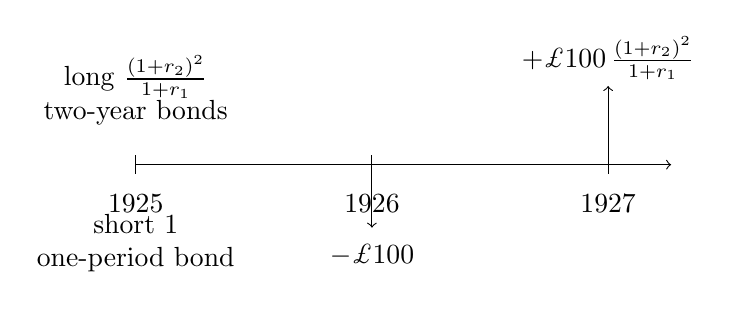
\begin{tikzpicture}[scale=1.0]
\draw[->] (0,0) -- (6.8,0);
\draw (0,0.12) -- (0,-0.12) node[below=4pt] {$1925$};
\draw (3,0.12) -- (3,-0.12) node[below=4pt] {$1926$};
\draw (6,0.12) -- (6,-0.12) node[below=4pt] {$1927$};
\node[align=center] at (0,0.95) {long $\frac{(1+r_2)^2}{1+r_1}$\\ two-year bonds};
\node[align=center] at (0,-1.0) {short $1$\\ one-period bond};
\draw[->] (3,0) -- (3,-0.8);
\node at (3,-1.15) {$-\pounds 100$};
\draw[->] (6,0) -- (6,1.0);
\node at (6,1.35) {$+\pounds 100\,\frac{(1+r_2)^2}{1+r_1}$};
\end{tikzpicture}
\caption{Timeline for the one-step forward-rate construction. The trade uses 1925 positions to lock in the gross return between 1926 and 1927.}
\end{figure}

Shiller then gives the identity its economic interpretation. Expectations theory says, in words, that the forward rate equals the expected future spot rate. In compact notation, one may write
\begin{equation}
f \approx \mathbb{E}_t\!\left[r^{\text{spot}}_{t+1}\right].
\end{equation}
The key phrase in the lecture is that the whole future seems to be laid out in this morning's paper. Once the term structure is observed, forward-rate formulas extract implied future one-period rates all along the horizon.

But Hicks immediately qualifies the pure expectations theory. Forward rates are not simply forecasts. They also contain risk compensation. In a cleaned analytic normalization,
\begin{equation}
f=\mathbb{E}_t\!\left[r^{\text{spot}}_{t+1}\right]+\pi,
\qquad
\pi>0.
\end{equation}
So forward rates tend to lie above optimally forecast future spot rates. The gap is the risk premium. This is the lecture's closing technical point.

\section{From the theory of interest to the problem of usury}

Only now does Shiller return to what he postponed near the start. The Fisher story makes lending look unambiguously welfare-improving. The loan market allows gains from trade. The term structure lays out rates for many horizons. The whole apparatus looks elegant and socially useful. Why, then, have religious and social traditions so often treated interest as dangerous or immoral?

The lecture answers by stepping back into the language of usury. The old Latin word usura can mean use, and it can also mean interest. More troublingly, it can shade into excessive or abusive interest. That ambiguity matters. Shiller does not try to settle biblical or Islamic exegesis. Instead he uses the ambiguity to make a conceptual point: suspicion of lending persists because in real life a difference in present and future consumption plans is not always an innocent difference in taste.

\subsection{Question \& Answer}

\paragraph{Question.} If lending raises welfare in the Fisher story, why has interest so often been condemned?

\paragraph{Answer.} Because in actual debt markets the borrower may be impatient in a harmful rather than a merely descriptive sense. The Fisher model treats a desire for present consumption as a preference. Real life may force a different judgment. The borrower may be making a mistake, acting on temptation, ignoring future distress, or responding to manipulation. In that case the right response may be advice or protection, not simply more credit. Usury, in the lecture's closing definition, is abusive lending undertaken without genuine concern for the borrower's welfare.

That is why Shiller brings behavioral economics back into the story. If one of the Crusoes wants to consume far too much today, perhaps the real issue is not that a loan has failed to appear. Perhaps the issue is that he should be told not to do it. Once we say that, the path from Fisher's clean geometry to the real world becomes less smooth.

The examples at the end of the lecture are chosen for exactly this reason. Vacation loans sound dubious. Yet Modigliani's remark about honeymoons complicates the matter: some expenditures that look like consumption may actually be investments in memory, relationship, and life trajectory. So the lecture refuses a simple moralism. It does not say that such loans are always wrong. It says that the real question is whether lenders are helping borrowers make good intertemporal choices or exploiting their vulnerabilities.

Elizabeth Warren enters at the close as the institutional form of this concern. Her work on bankruptcy, household distress, and abusive lending practices is used to show that modern debt markets can systematically harm people while appearing, on the surface, to offer them choice. The Consumer Financial Protection Bureau appears in the lecture as a modern answer to a very old problem. We do not reject lending. We regulate it.

This is the balance Shiller wants to keep. The original Fisher and Bohm-Bawerk story about interest was basically right. Even apparently soft loans, including honeymoon loans, are not automatically illegitimate. But the old suspicion of usury is not empty rhetoric. It survives because lending can become predatory, and because a useful debt market still needs government rules against abuse.

\section{Summary}

The lecture begins with a puzzle and ends with a distinction. The puzzle is why interest exists at all and why it is positive and modest in scale. The distinction is between useful debt and abusive debt. In between, the lecture unfolds step by step. Bohm-Bawerk offers the old verbal causes. Fisher turns them into a two-period geometry in which technology and preferences jointly determine the interest rate. The arithmetic of finance then carries that rate into discount-bond pricing, compounding conventions, present discounted value, perpetuities, annuities, and conventional bonds. Forward rates show that the term structure already contains prices for future intervals, though not without risk premia. And only then does the lecture return to the moral question. Lending is not repudiated. It is defended, but defended with the important qualification that real borrowers are behaviorally fragile and that debt markets need regulation against usury.